%%%%%%%%%%%%%%%%%%%%%%%%
% Compile with XeLaTeX %
%%%%%%%%%%%%%%%%%%%%%%%%

\documentclass{beamer}
    % Beamer settings
    \usetheme{Warsaw}
    \usefonttheme{professionalfonts}
    \usefonttheme{serif}
    % Packages and settings
    \usepackage{fontspec}
        \setmainfont{Charis SIL}
    \usepackage{graphicx}
        \graphicspath{{../figures/}}
    % Document information
    \title{Chapter 8: Language Acquisition}
\begin{document}
    \begin{frame}
        \titlepage
    \end{frame}
    \begin{frame}
        \tableofcontents
    \end{frame}
    \AtBeginSection[]
        {
        \begin{frame}
            \tableofcontents[currentsection]
        \end{frame}
        }
    \section{Introduction}
        \begin{frame}{What is language acquisition?}
            \begin{itemize}
                \item<2-> Starting to speak for the first time
                    \begin{itemize}
                        \item<3-> Referred to as \alert{first-language acquisition}
                    \end{itemize}
                \item<2-> Picking up a new language in college
                    \begin{itemize}
                        \item<3-> Referred to as \alert{second-language acquisition (SLA)} or second-language learning
                    \end{itemize}
            \end{itemize}
        \end{frame}
    \section{Theories of language acquisition}
        \begin{frame}{What must children acquire?}
            \begin{itemize}
                \item Words
                    \begin{itemize}
                        \item Can potentially learn through memorization
                    \end{itemize}
                \item Rules of the grammar
                    \begin{itemize}
                        \item Includes phonology, morphology, and syntax
                        \item \emph{Cannot} simply be memorized
                    \end{itemize}
            \end{itemize}
            \begin{example}<2->
                What sort of words can the prefix \emph{un-} attach to? How did you learn this?
            \end{example}
        \end{frame}
        \begin{frame}{Some theories}
            \begin{itemize}
                \item \alert<2->{The innateness hypothesis}
                \item Imitation theory
                \item Reinforcement theory
                \item Active construction of a grammar theory
                \item Connectionist theories
                \item Social interaction theory
            \end{itemize}
        \end{frame}
        \begin{frame}{The innateness hypothesis}
            \begin{block}{Definition}
                The idea that humans are genetically predisposed to acquire and use language
            \end{block}
            \begin{itemize}
                \item<2-> Babies are born knowing that languages have patterns (and possibly features).
                \item<2-> Babies are born with the ability to seek out those patterns (and possibly features).
                \item<2-> The collection of all possible patterns together is known as \alert{universal grammar}.
            \end{itemize}
            \begin{example}<3->
                All languages might have nouns and verbs.
            \end{example}
        \end{frame}
        \begin{frame}{The innateness hypothesis}
            What are some innate behaviors?
            \begin{itemize}
                \item<2-> Walking
                \item<2-> Eating
            \end{itemize}
            What are some learned behaviors?
            \begin{itemize}
                \item<3-> Playing piano
                \item<3-> Riding a bike
            \end{itemize}
            \begin{alertblock}<4->{}
                Is talking like walking and eating or is it like playing the piano and riding a bike?
            \end{alertblock}
        \end{frame}
        \begin{frame}{The innateness hypothesis}
            Eric Lenneberg's characteristics of innate behaviors can help us answer this question:
            \begin{enumerate}
                \item The behavior emerges before it is necessary
                \item<2-> Its appearance is not the result of a conscious decision
                \item<3-> Its emergence is not triggered by external events (but the environment must be ``rich'')
                \item<4-> Direct teaching and intensive practice have \emph{relatively} little effect
                \item<5-> The behavior develops through identifiable and ordered stages
                \item<6-> There is likely a \alert{critical period} for acquiring the behavior
            \end{enumerate}
        \end{frame}
        \begin{frame}{The innateness hypothesis}
            Does direct teaching really have little effect?
            \begin{example}
                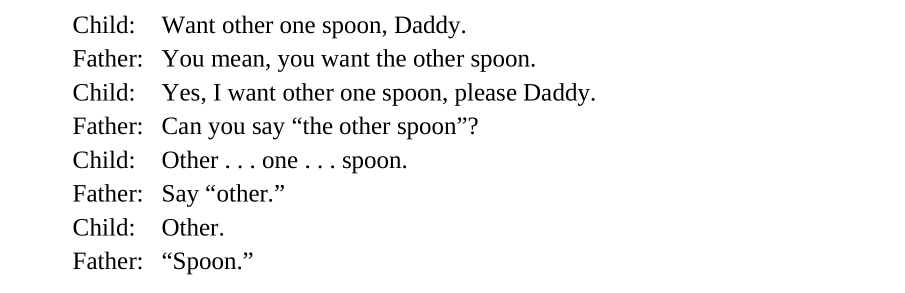
\includegraphics[scale=0.45]{DirectTeaching.PNG}

                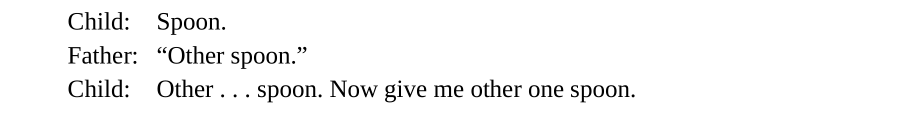
\includegraphics[scale=0.445]{DirectTeaching2.PNG}
            \end{example}
        \end{frame}
        \begin{frame}{The innateness hypothesis}
            \begin{block}{Definition of a \alert{critical period}}
                A period of time during which a behavior must be acquired.
            \end{block}
            \begin{itemize}
                \item<2-> Acquisition cannot occur before or after this period
                \item<2-> For language acquisition: \alert{birth to the onset of puberty}
            \end{itemize}
            \uncover<3->{How did we figure out when the critical period for language acquisition is?}
            \begin{itemize}
                \item<4-> Neglected children and \alert{feral children}
            \end{itemize}
        \end{frame}
        \begin{frame}{The innateness hypothesis}
            \begin{example}
                Genie and Isabelle:
                \begin{itemize}
                    \item Genie was kept in isolation from the age of 20 months until the age of 13
                    \begin{itemize}
                        \item<2->[$\rightarrow$] Never acquired language
                    \end{itemize}
                    \item Isabelle was kept in isolation until the age of 6
                    \begin{itemize}
                        \item<2->[$\rightarrow$] Language skills caught up to those of other children her age after 2 years of lessons
                    \end{itemize}
                \end{itemize}
            \end{example}
            \uncover<3->{What might be some issues with this evidence for the critical period?}
            \begin{itemize}
                \item<4-> Genie was abused and traumatized
                \item<4-> Isabelle used a rudimentary \alert{homesign} gestures with her deaf mother
            \end{itemize}
        \end{frame}
        \begin{frame}{The innateness hypothesis}
            \begin{block}{Definition of \alert{homesign} gestures}
                Gestures that represent common actions and objects (e.g., `eat' or `house') but that do not involve grammatical rules
            \end{block}
            \begin{alertblock}<2->{}
                What do these have to do with evidence for the innateness of language?
            \end{alertblock}
        \end{frame}
        \begin{frame}{The innateness hypothesis}
            \begin{example}
                In the 1980s, a school for the deaf was established in Nicaragua:
                \begin{itemize}
                    \item Both young and old students arrived knowing only homesign gestures
                    \begin{itemize}
                        \item[$\rightarrow$] Students standardized their homesign gestures
                        \begin{itemize}
                            \item[$\rightarrow$] Later, young students developed a full-blown sign language through their exposure
                        \end{itemize}
                    \end{itemize}
                \end{itemize}
                \uncover<2->{Older students in the first generation never moved beyond homesign gestures.}
            \end{example}
        \end{frame}
        \begin{frame}{The innateness hypothesis}
            Second-language acquisition presents both evidence for and against the critical period:
            \begin{itemize}
                \item<2-> Adult second language learners \emph{rarely} learn a new language perfectly
                \item<2-> Child second language learners \emph{regularly} learn a new language perfectly
                    \uncover<3->{
                        \begin{itemize}
                            \item \emph{BUT}
                        \end{itemize}
                        }
                \item<3-> Some adults \emph{can} learn a new language perfectly
                \item<3-> Factors such as teaching methods, motivation, and identity are difficult to control for
            \end{itemize}
        \end{frame}
        \begin{frame}{The innateness hypothesis}
            Different parts of the grammar also work differently:
            \begin{itemize}
                \item Feral children can learn vocabulary but not syntax
                \item Second language learners can learn vocabulary and syntax but not phonology
            \end{itemize}
            \begin{alertblock}{}
                Therefore, perhaps only certain parts of language are innate
            \end{alertblock}
        \end{frame}
        \begin{frame}{Imitation theory}
            \begin{alertblock}{}
                Innateness theory does not say much about \emph{how} language is acquired
            \end{alertblock}
            \begin{block}<2->{Definition of \alert{imitation theory}}
                The idea that children acquire language by listening to the speech around them and reproducing what they hear
            \end{block}
            \begin{alertblock}<3->{}
                Does this sound reasonable?
            \end{alertblock}
        \end{frame}
        \begin{frame}{Imitation theory}
            The truths of this theory:
            \begin{itemize}
                \item The connection between words and their meaning is arbitrary
                \begin{itemize}
                    \item[$\rightarrow$] Must be learned through imitation
                \end{itemize}
                \item<2-> Children learn languages in their environment, not those that are absent
                \begin{itemize}
                    \item<2->[$\rightarrow$] On some level, they are attempting to imitate what they hear
                \end{itemize}
            \end{itemize}
        \end{frame}
        \begin{frame}{Imitation theory}
            But still... \uncover<2->{this child is producing something they've never heard and is refusing to imitate what they do hear.}
            \begin{example}
                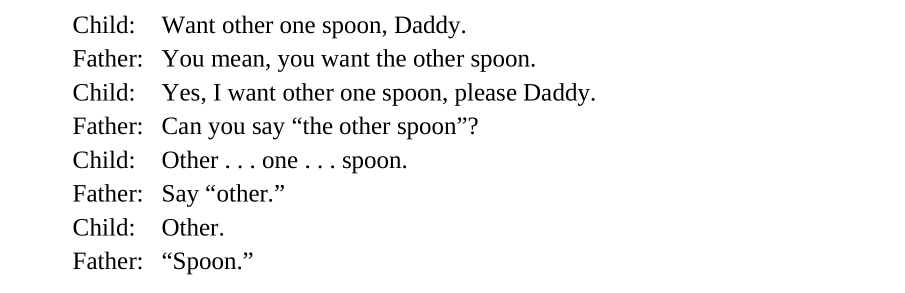
\includegraphics[scale=0.45]{DirectTeaching.PNG}\\
                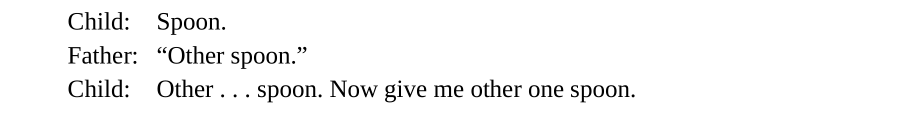
\includegraphics[scale=0.445]{DirectTeaching2.PNG}
            \end{example}
        \end{frame}
        \begin{frame}{Reinforcement theory}
            \begin{block}{Definition}
                The idea that children learn language by being rewarded when using correct forms and being corrected when using incorrect forms
            \end{block}
            \begin{alertblock}<2->{}
                Does this sound reasonable?
            \end{alertblock}
        \end{frame}
        \begin{frame}{Reinforcement theory}
            \begin{example}
                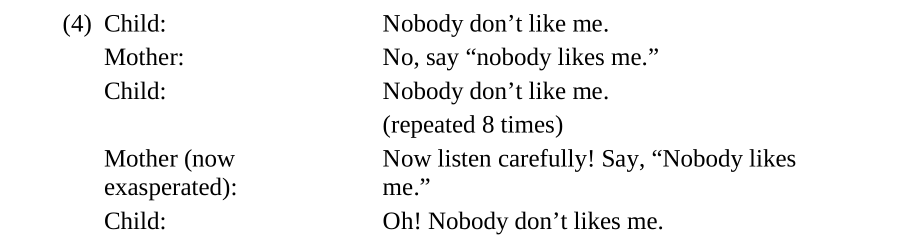
\includegraphics[scale=0.45]{Correcting.PNG}
            \end{example}
            \begin{itemize}
                \item<2-> Most corrections are for the truth value
                \item<2-> Corrections aren't always heeded
            \end{itemize}
        \end{frame}
        \begin{frame}{Active construction of a grammar theory}
            \begin{block}{Definition}
                The idea that language acquisition is innate, and children hypothesize about rules for patterns they hear, eventually inventing their own grammar
            \end{block}
            \begin{alertblock}{}
                This differs from the innateness hypothesis in that the patterns themselves \emph{are not} innate.
            \end{alertblock}
        \end{frame}
        \begin{frame}{Active construction of a grammar theory}
            \begin{example}
                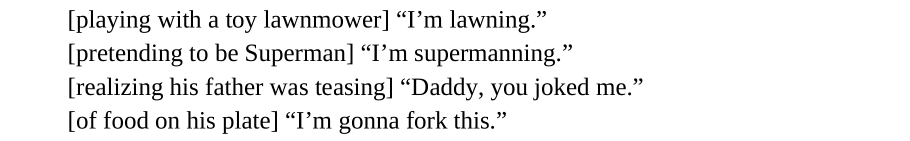
\includegraphics[scale=0.45]{Lawning.PNG}
            \end{example}
            \begin{alertblock}<2->{}
                These mistakes are non-random; they stem from the child's own, invented, unrefined rules.
            \end{alertblock}
        \end{frame}
        \begin{frame}{Connectionist theories}
            \begin{block}{Definition}
                The idea that children develop neural connections in the brain via their exposure to and use of language in different circumstances
            \end{block}
            \begin{example}<2->
                Circumstance: a child hearing the word `milk' while drinking from a bottle\\
                Association: `milk' to the sound of the word\\
                Association: `milk' to the image of a bottle\\
                Association: `milk' to drinking\\
            \end{example}
        \end{frame}
        \begin{frame}{Connectionist theories}
            These theories differ from active construction of a grammar theory:
            \begin{itemize}
                \item Active construction of a grammar suggests that children create categorical, abstract rules
                \item Constructionist theories suggest that children exploit statistics and probability to guess what form to use
            \end{itemize}
            \begin{example}<2->
                Children do not always use \emph{-ed} to create the past tense of nonsense words like `fring'.
            \end{example}
            \begin{itemize}
                \item<3-> Active construction of a grammar theory can't explain this
                \item<3-> Constructionist theories explain this by saying that forms like `frang' are more likely here because of `sing', `ring', and `bring'
            \end{itemize}
        \end{frame}
        \begin{frame}{Social interaction theory}
            \begin{block}{Definition}
                The idea that children cue adults for the sort of language input they require in order to develop grammatical rules
            \end{block}
            \begin{example}<2->
                Children are much more likely to hear (5) than (6):
                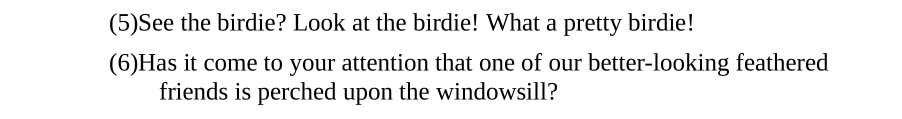
\includegraphics[scale=0.45]{Birdie.PNG}
            \end{example}
            \begin{alertblock}<3->{}
                This theory is not necessarily in opposition to other theories.
            \end{alertblock}
        \end{frame}
    \section{Practice}
        \begin{frame}{How do these theories apply here?}
            \begin{itemize}
                \item \url{https://youtu.be/22aMls0Cg-A?t=2}
                \item \url{https://youtu.be/2uaBTKes0Ok}
                \item \url{https://youtu.be/uOpXNhNqGJw}
                \item \url{https://youtu.be/UrRKLHq25UA?t=135}
            \end{itemize}
        \end{frame}
\end{document}
